%% -----------------------------------------------------------------------------


The test bed for executing the experimental process utilizes a machine with two
Intel Xeon Gold 6258R processors (28 doubly-threaded cores each) and 500GB of
memory.  Each debugging scenario had a 4 minute timeout and a 6GB memory
limit. Running the experiment on all debugging scenarios took over
30,000 compute hours or roughly three-and-a-half compute years. 

\
\begin{figure} \footnotesize 
  \centering
  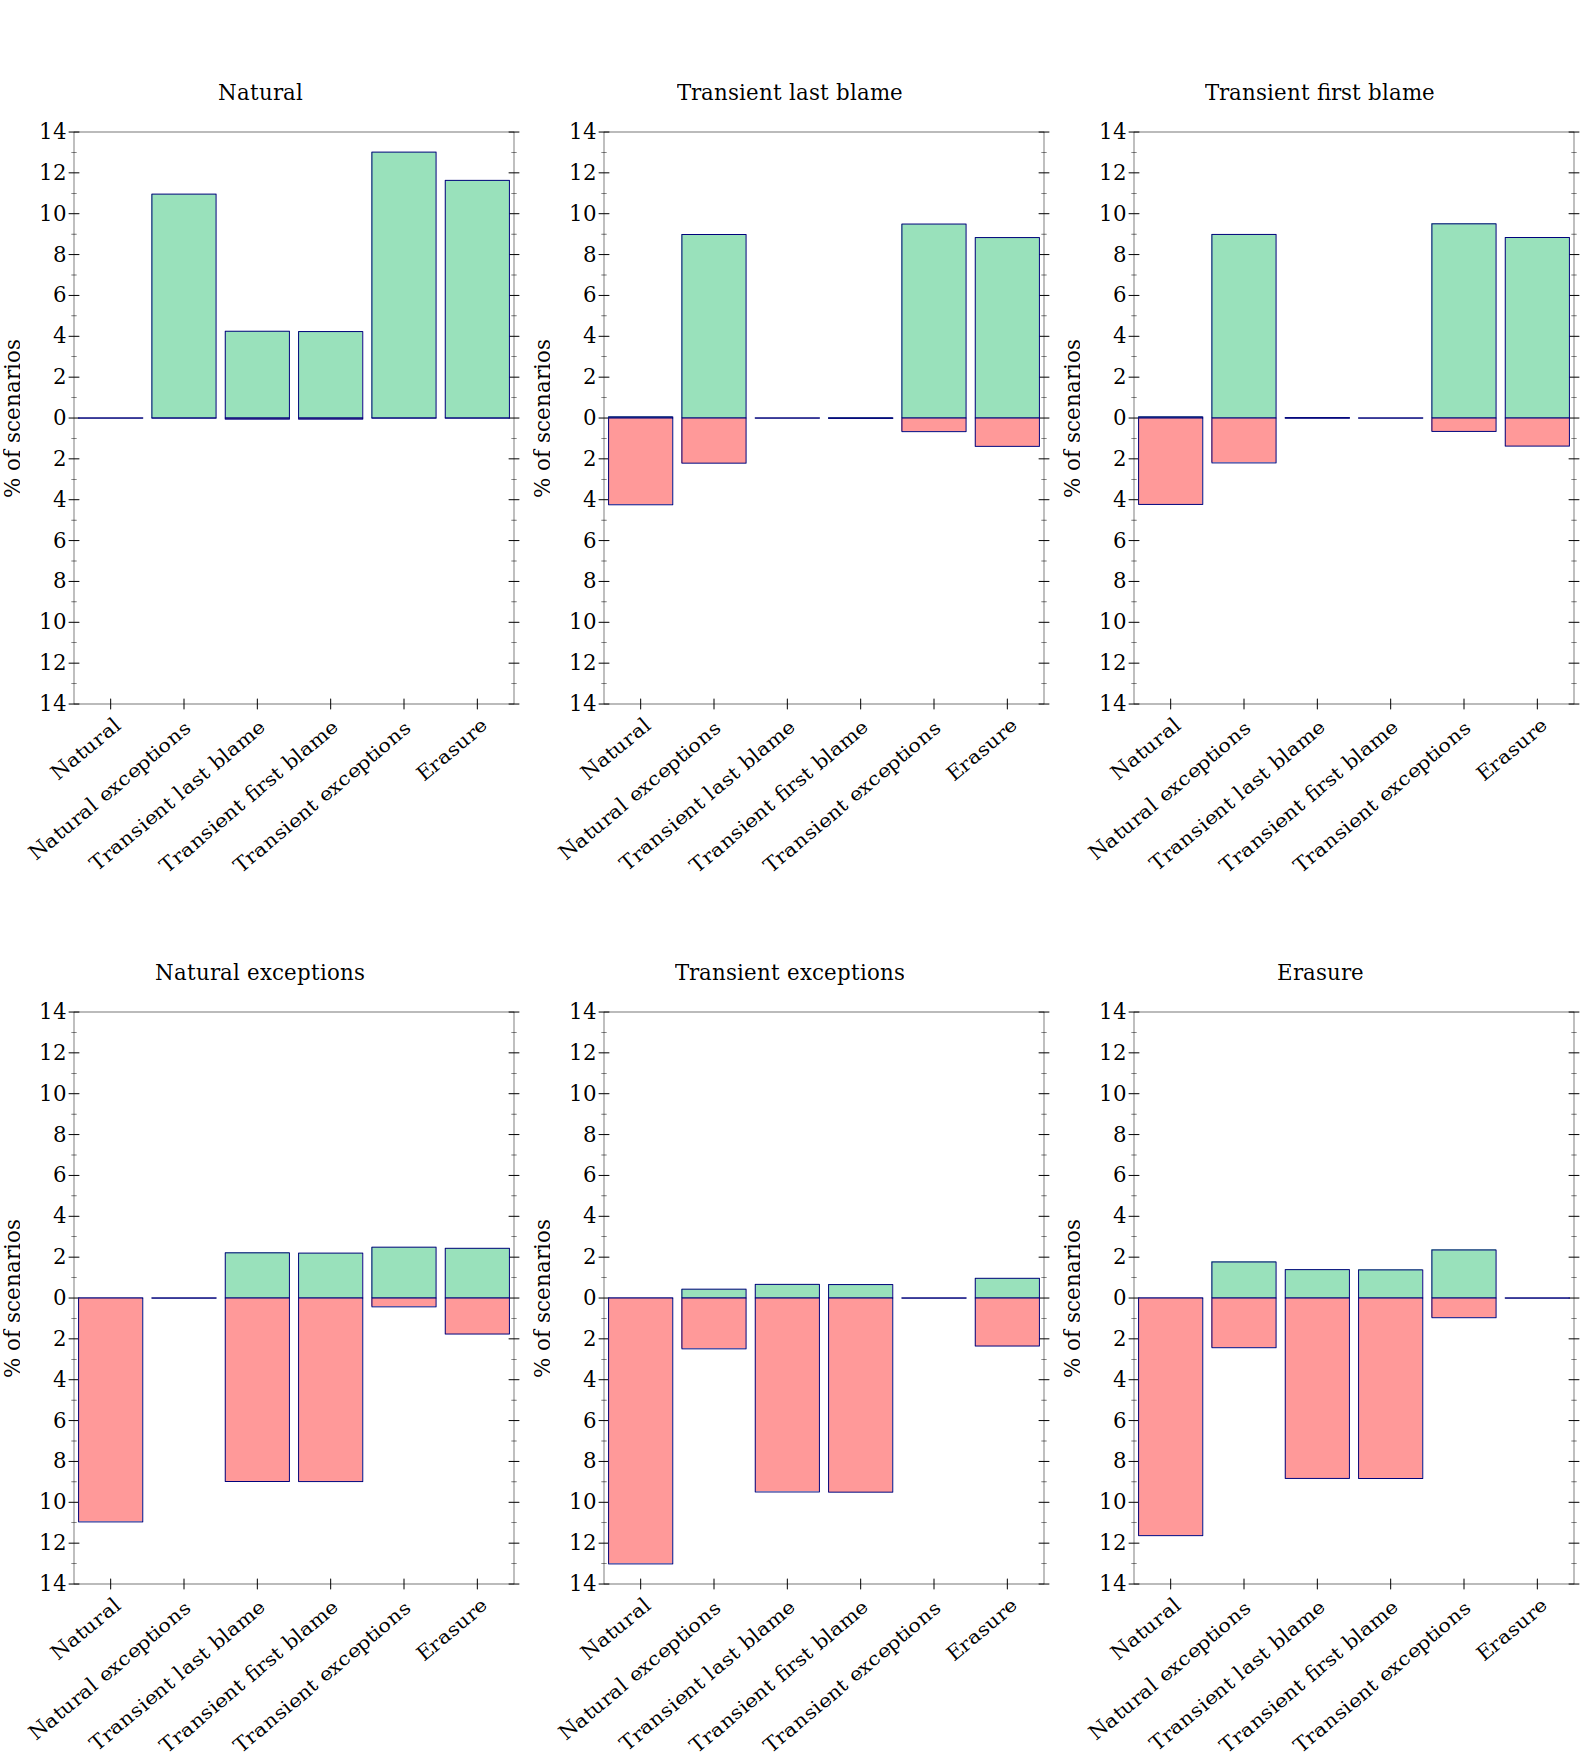
\includegraphics[width=\textwidth]{./plots/avo-bars}

  \vspace{1em}
  \begin{minipage}{0.95\textwidth}
      Each plot depicts a head-to-head comparison of the mode named above the
      plot vs. every other mode.  The (green) portion above 0 is the estimated
      percentage of scenarios where the named mode is more useful than the
      other.  The (red) portion below 0 is the estimated percentage of scenarios
      where the named mode is less useful than the other.  The upper bound
      margin of error is 0.02\%.
  \end{minipage}

  \caption{Usefulness comparisons}
  \label{fig:avo-bars}
\end{figure}

\begin{figure}\footnotesize 
  \centering
  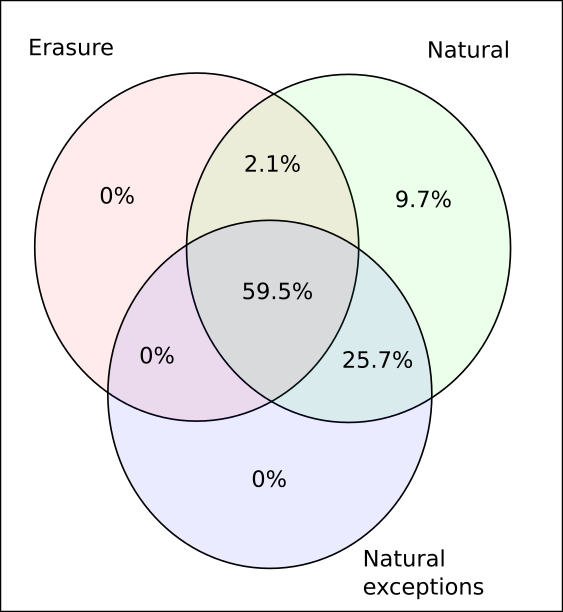
\includegraphics[width=0.32\textwidth]{./plots/TR-TR-stack-first-venn}
  \hfill
  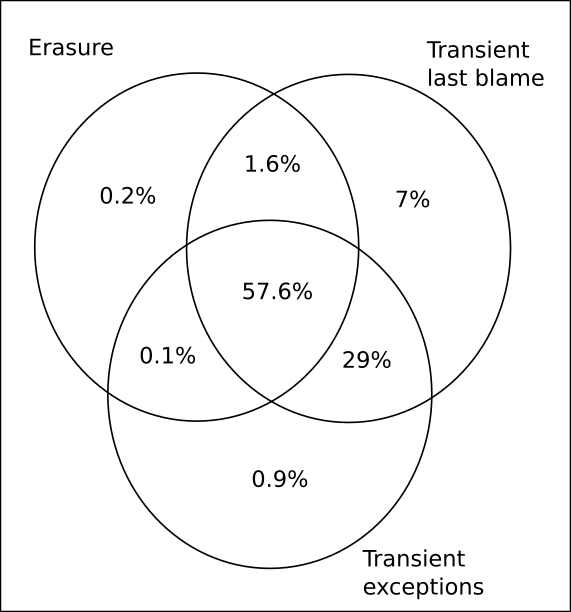
\includegraphics[width=0.32\textwidth]{./plots/transient-newest-transient-stack-first-venn}
  \hfill
  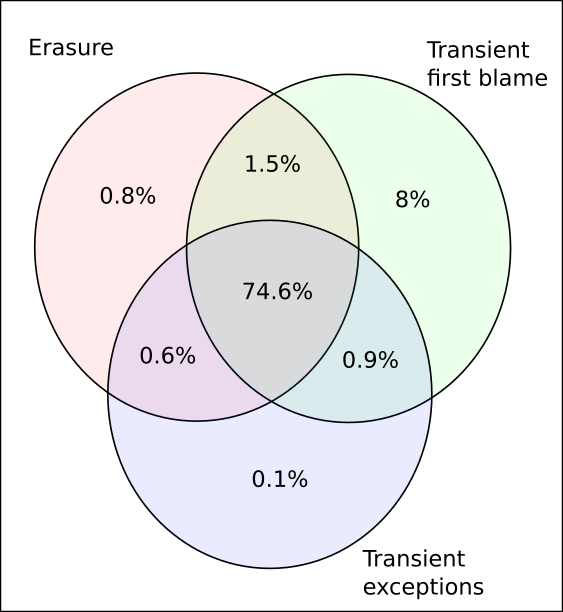
\includegraphics[width=0.32\textwidth]{./plots/transient-oldest-transient-stack-first-venn}

  \vspace{1em}
  \begin{minipage}{0.95\textwidth}

     Each diagram shows the overlap of the successful scenarios for three modes.
     For example, in the leftmost diagram, all three modes succeed on the same
     scenario 57.3\% of the time, only Natural and Natural exceptions succeed on
     29.1\% of the scenarios, only Natural and Erasure succeed on 2.1\%, and
     Natural alone succeeds on 9\%. The upper bound margin of error is 0.02\%.

  \end{minipage}

  \caption{Blame usefulness analysis}
  \label{fig:success-venns}
\end{figure}


% \footnote{The random mode behaves the same for all three semantics, so this analysis considers it a single mode.}

\begin{wrapfigure}{r}{.40\textwidth} \footnotesize 
  \vspace{-1.5em}
  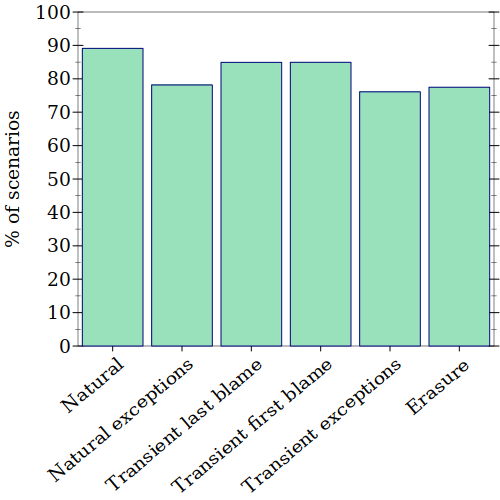
\includegraphics[width=0.38\textwidth]{./plots/success-bars}
  \vspace{1em}
  \begin{minipage}{0.35\textwidth} \raggedright
%   The estimated percentage of scenarios for which each mode succeeds in locating the bug.
   The upper bound margin of error is 0.02\%.
  \end{minipage}
\vspace{-2em}
  \caption{Percentage rates of success} \label{fig:success-bars}
\end{wrapfigure}



Figure~\ref{fig:success-bars} summarizes the overall success rates of
every mode.
The success rates illustrate a few points that underlie the
rest of the analysis.  The first notable piece of information from this
figure is that every mode has failed debugging scenarios, not just
Erasure. This should not come as a surprise to the astute reader.  Running
a rational programmer mode on a scenario may result in an exception
that carries no useful information about which module to equip with types next. For instance the stack trace of the exception may not
contain frames from any untyped module of the program. This can happen at any point
along a blame trail, causing it to fail.

While most blame trail failures follow the above pattern, a few do
not.  Breaking down the failure reasons for Natural blame (1748 in
total) reveals an additional cause. For a small set of debugging scenarios
(40), Natural produces a run-time type error blaming a non-buggy
already-typed module. All these cases are due to known open issues with Typed
Racket and class contracts. 

In Transient, similar to Natural, most failures are due to unhelpful exception
information (1851 for both Transient first and last blame).  However, Transient
also has a substantial number of failures because scenarios hit the time and/or
memory limits of the experiment (\textasciitilde770 scenarios).  Additionally,
there are nearly 1,000 cases where Transient reports an empty blame set, leaving
the rational programmer without hints about how to proceed.
Sections~\ref{sec:threat:transient} and ~\ref{sec:threat:transient2} address
these causes of failure for Transient and how they affect the experiment.

The second key observation from figure~\ref{fig:success-bars} is that the modes
that use blame all outperform those that do not. In particular, Natural and both
of Transient's blame modes succeed in 85 - 90\% of the scenarios, while their
corresponding exception modes succeed in less than 80\% of them, and so too for
Erasure. The only exception is that the random programmer always succeeds; the
figure omits this mode because it just reflects the fact that every scenario has
finitely many modules, so the random programmer eventually types the buggy
module.

Figure~\ref{fig:avo-bars} depicts a head-to-head comparison of every
mode's performance against every other mode (except Random). The
comparison  answers the four questions from section~\ref{sub:experiment}. 
Each plot shows the proportion of scenarios where one mode performs
better or worse than each other mode.  In particular, each bar above zero
represents the proportion where the plot's named mode succeeds and the
mode on the x-axis fails; the corresponding bar below zero represents the
proportion of the inverse case.  For example, the plot titled ``Natural''
shows that Natural outperforms Natural exceptions in about 11\% of the
scenarios, and the inverse (Natural performs worse than Natural
exceptions) never happens.  Similarly, the plot titled ``Transient last
blame'' shows that Transient last blame outperforms Natural exceptions
 in about 9\% of the scenarios, but conversely it performs worse
than Natural exceptions in about 2\% of the scenarios.

The figure answers questions $Q_1$, $Q_2$ and $Q_3$ affirmatively.  
In all three semantics, blame modes outperform their
corresponding exception mode by \textasciitilde10\%.  The
Natural exceptions mode is never more useful than Natural blame, and
Transient exceptions are more useful than Transient first and Transient
last blame in a small percentage (less than 1\%) of the scenarios. 

Figure~\ref{fig:avo-bars} also provides answers for $Q_*$. Blame for all three
semantics is significantly more useful than Erasure exceptions---by almost
12\% for Natural and almost 9\% for Transient. Natural blame is more useful than
both versions of Transient blame by a small percentage (about 4\%). The
Transient first and Transient last blame are practically indistinguishable.
Finally, Natural exceptions are more useful than Transient exceptions, although
only in a small percentage of scenarios (about 2.5\%). A rare few scenarios
(about 0.5\%) show the opposite, despite the theoretically advantageous
additional checks of Natural.

\begin{figure} \footnotesize \centering
  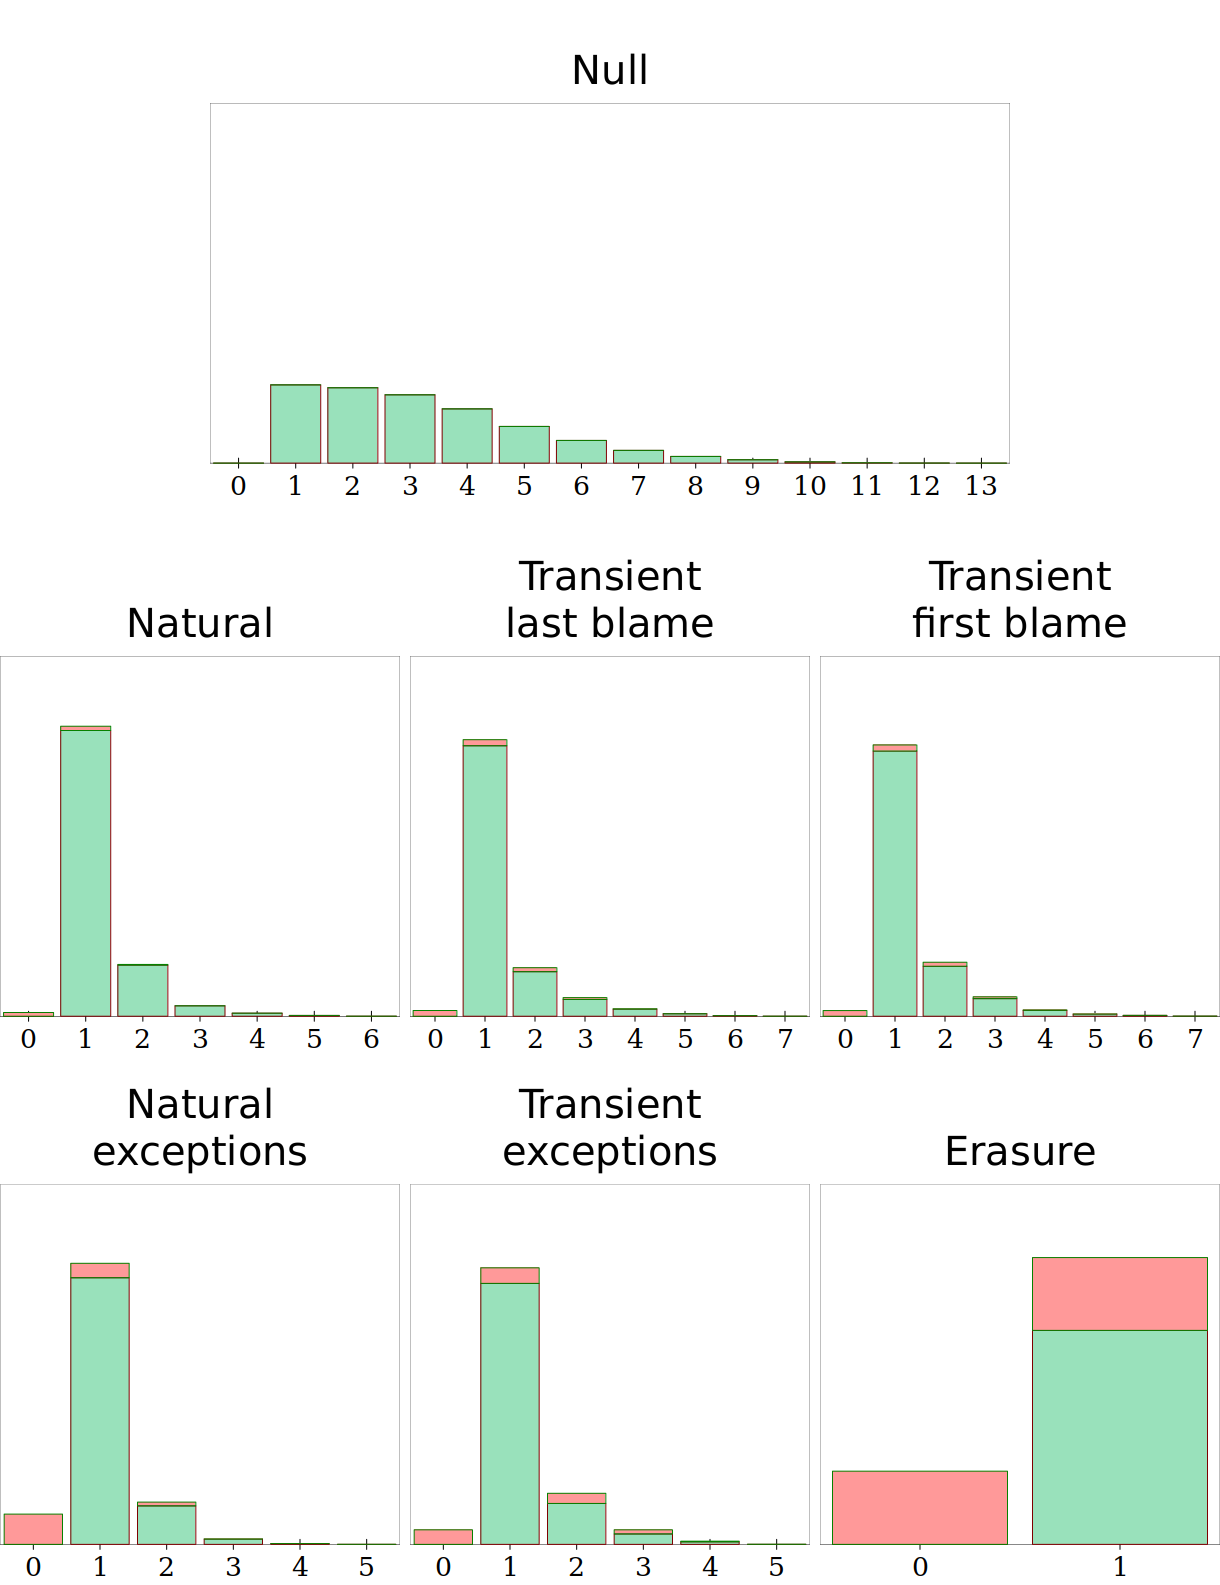
\includegraphics[width=\textwidth]{./plots/bt-lengths-table}

  \vspace{1em}
  \begin{minipage}{0.95\textwidth}
    Each plot depicts the distribution of trail lengths for a given mode across all benchmarks.
    The upper bound margin of error is 0.05\%.
  \end{minipage}

  \caption{Programmer effort} \label{fig:effort-table}
\end{figure}

\begin{figure}\footnotesize \centering
  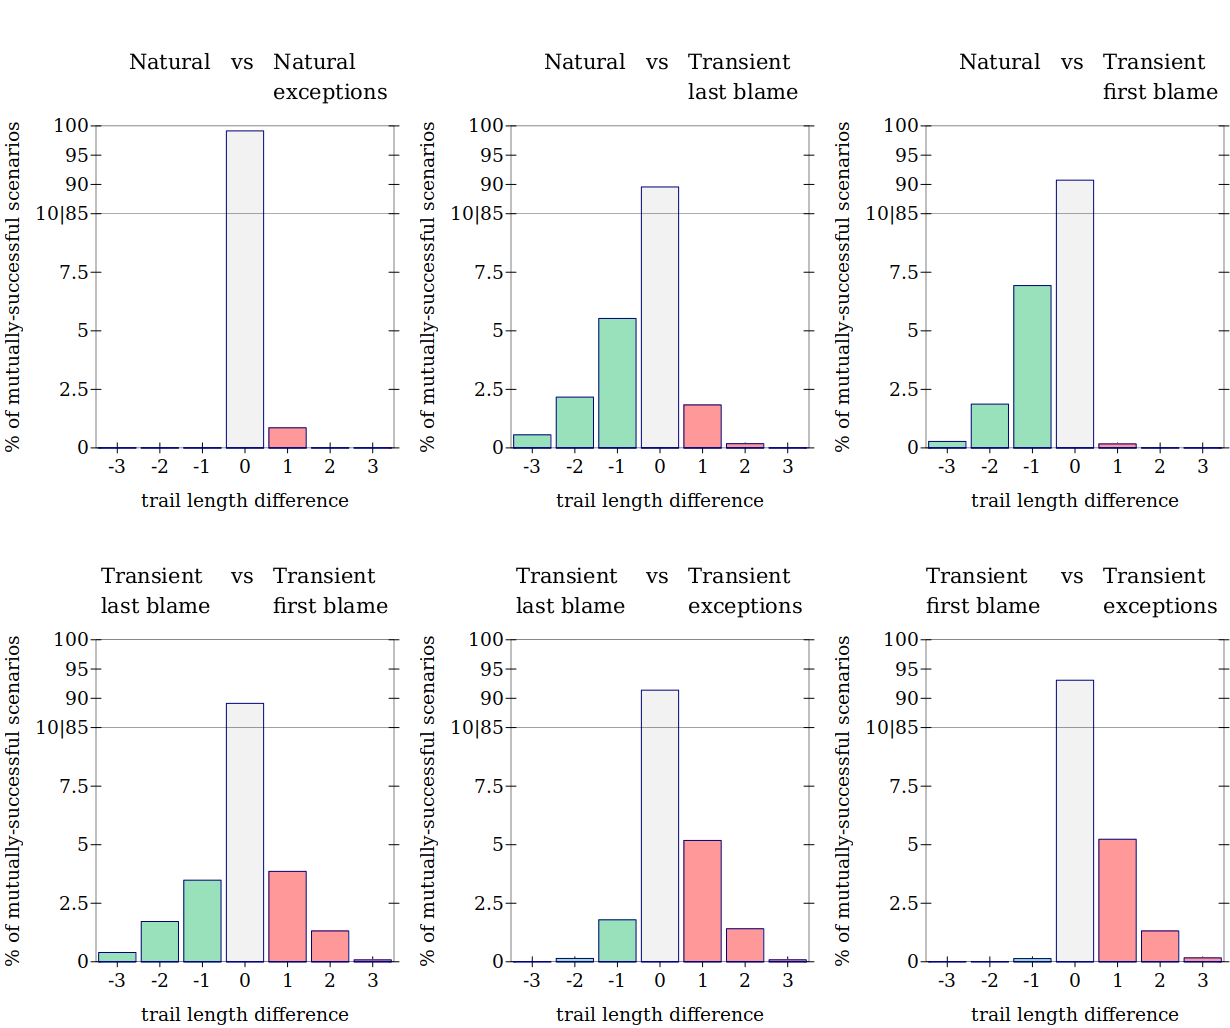
\includegraphics[width=\textwidth]{./plots/bt-length-comparisons}

  \vspace{1em}
  \begin{minipage}{0.95\textwidth}

    Each plot depicts the distribution of scenarios with trail length
    differences ranging from -3 to 3. A $-x$ difference denotes that the first
    mode's trail is $x$ steps {\em shorter\/} than the second mode's trail for the
    same scenario; a positive difference denotes the inverse. A difference of
    $\infty$ indicates one mode's trail succeeds while other mode's fails. The
    15|60 on the y-axis indicates that the axis is truncated between 15 and
    60\%.
    The upper bound margin of error is 0.03\%.

  \end{minipage}

  \caption{Effort comparisons} \label{fig:effort-comparisons}
\end{figure}

An alternative way to understand the answers for questions $Q_1$ to $Q_3$, is to
analyze the success of each semantics in comparison to
Erasure. Figure~\ref{fig:success-venns} depicts the results of this analysis.
Specifically, the figure shows one Venn diagram per mode of the rational
programmer that uses blame.  Each diagram shows the overlap of successful
scenarios for the blame mode, its corresponding exception mode, and Erasure.
For example, the leftmost diagram (Natural) shows that all three modes succeed
on 75.7\% of the scenarios, only Natural and Natural exceptions succeed on
11.6\% of the scenarios, only Natural and Erasure succeed on 1.8\%, and Natural
alone succeeds on 9.2\%.  This analysis highlights the success trade-offs each
semantics offers against Erasure, with and without blame. For instance, the
analysis for Natural clearly illustrates that, when choosing between Natural
blame, Natural exceptions, and Erasure, Natural blame is the absolutely most
successful: all of the successes of the other two modes are subsets of Natural's
successful scenarios.  On the other hand, Transient's blame modes fare similarly
but the choice is not so clear-cut.

Turning to programmer effort, figure~\ref{fig:effort-table} shows the
estimated distribution of blame trail lengths for the interesting debugging
scenarios. There are two immediate take-aways from the figure. First, the effort for
successfully debugging interesting scenarios (in green) for the random
mode of the rational programmer is highly spread out, as
expected. In contrast, in the other modes, successful effort coalesces at
the left side of the plot, meaning that in most cases the programmer needs
to type a single module to debug a scenario. 

Second, the exceptions of the Erasure semantics either help the rational
programmer immediately or the rational programmer fails to debug a scenario
altogether (in red).  This is expected; adding type annotations to an Erasure
program does not change its behavior, so if the type checker does not reject the
program with the new annotations, the rational programmer is stuck.  In other
words, an exception from the run-time system has to point to the buggy module with the
first try. Otherwise the rational programmer types an irrelevant module, runs
the program again, and the same exception points again to the already typed
module.

Figure~\ref{fig:effort-comparisons} provides head-to-head comparisons of effort.
The comparison between two modes boils down to the difference in length between
their trails for all scenarios where they both succeed. Hence, each plot in the
figure shows the distribution of scenarios with length differences ranging from
-3 (the first mode's trail is 3 steps shorter than the second's) to 3 (the first
mode's trail is 3 steps longer than the second's). The figure offers several
insights about how modes compare in terms of effort that complement the insights
about how they compare in terms of success rates from figure~\ref{fig:avo-bars}.
First, Natural blame never produces shorter trails than Natural exceptions, and
sometimes (albeit rarely) produces slightly longer ones. Hence, the experiment
provides evidence that blame helps the rational programmer debug more scenarios
but does not shorten the debugging process compared to exceptions. Second,
Natural relatively often (close to 8\% of the scenarios) produces shorter trails
than both Transient blame modes, and sometimes the trails are significantly
shorter. Finally, Transient's blame modes also share the characteristic with
Natural that blame sometimes produces longer trails than their corresponding
exception modes.

